\documentclass{article}
% \usepackage[utf8]{inputenc}
\setlength{\parskip}{\baselineskip}%
\setlength{\parindent}{0pt}%


\title{Case Study for Insurance Modeling}
\author{Jinhuizi (Jeanne) Fu}
\date{\today}

\usepackage{natbib}
\usepackage{graphicx}

\begin{document}

\maketitle

\section{Introduction}
This case study will focus on pricing strategies for a commercial auto line of business. The goal of the study is to incorporate Machine Learning to improve pricing accuracy, while maintain explainability.

Throughout the life cycle of a insurance pricing project, there are in general six steps, and we will discuss in more detail how to use ML in each step:

\begin{itemize}
    \item Scoping (Set up a goal for the project, success criteria and/or metrics, resource, cost, etc.)
    \item Data Preparation (Data sourcing, EDA, data cleaning)
    \item Feature Engineering (Transformation, variable selection)
    \item Modeling (Benchmarking, feature importance ranking, model, validation)
    \item Implementation (Deploy model for business end-users, testing)
    \item Monitoring (and prepare for model refreshing)
\end{itemize}

This case study will be focusing on Data Preparation, Modeling and Implementation. I will discuss about potential risks and how to manage them in the end.

\section{Data Preparation}
In general, when preparing a modeling dataset for a pricing model, we will put together both internal and external data sources, and prepare for modeling data.

Internal data source:
\begin{itemize}
    \item Policy data: account/policy information, exposure, location, primary usage of vehicle, business industry, etc.
    \item Loss data: (Target, loss history). Loss linkage may be needed. 
    \item Vehicle information: vehicle weight, vehicle age, vehicle cost, etc. May use external VIN decoding service if needed.
\end{itemize}

External data source:
\begin{itemize}
    \item Driver information (credit history, police driving record, etc.)
    \item Credit history (for the business)
\end{itemize}

In this case, I downloaded a toy dataset as a quick sample to explore different modeling methods. The source is from this website: https://data.mendeley.com/datasets/5cxyb5fp4f/1 

Things to do when I have more time:
\begin{itemize}
    \item Explore missing values. Check why they are missing, either back fill with distribution, or define new "Missing" category.
    \item Check distribution and transform if needed
\end{itemize}

\section{Feature Engineering}

A lot of explorations could be done here. Include but not limited to:
\begin{itemize}
    \item Encoding catergorical variables
    \item Normalization for certain variables. For example, normalize historical claim count by a variable accounting for policy size, will help isolate the feature from account size.
    \item Explore feature interaction
    \item Bin numerical variables, and/or explore polinomial trend
\end{itemize}


\section{Model Training and Validation}

* Split Training, Test, Holdout (or Cross Validation)

* Selection of Target variables: Frequency and Severity VS. Pure Premium


Things to think about:
\begin{itemize}
    \item Different coverages
    \item Outlier in pure premium
    \item Need to develop loss (alternative is to use policy year as control variable)
    \item Need to trend
\end{itemize}

\subsection{AutoML for model Benchmarking} 

AutoML (automated machine learning) is a framework to run machine learning models automatically. For insurance pricing, because of regulation restrictions, GLM is still the most used model structure due to its simplicity and explainability. However, AutoML framework can be used as a first step in pricing models. 

A few ways to use AutoML in pricing model:
\begin{itemize}
    \item Model benchmarking: AutoML can run multiple machine learning models at one time, so we can compare the performance of different models.
    \item Variable importance ranking: Shapley plot can be used to explore variable importance.
    \item Partial dependence plot: like traditional one-way plot for each features VS target variable, we can examine the upward/downward trend when the feature increases/decreases.
\end{itemize}
 
\subsection{AutoML for model variable importance (Shapeley Value)} 

\begin{figure}[h!]
\centering
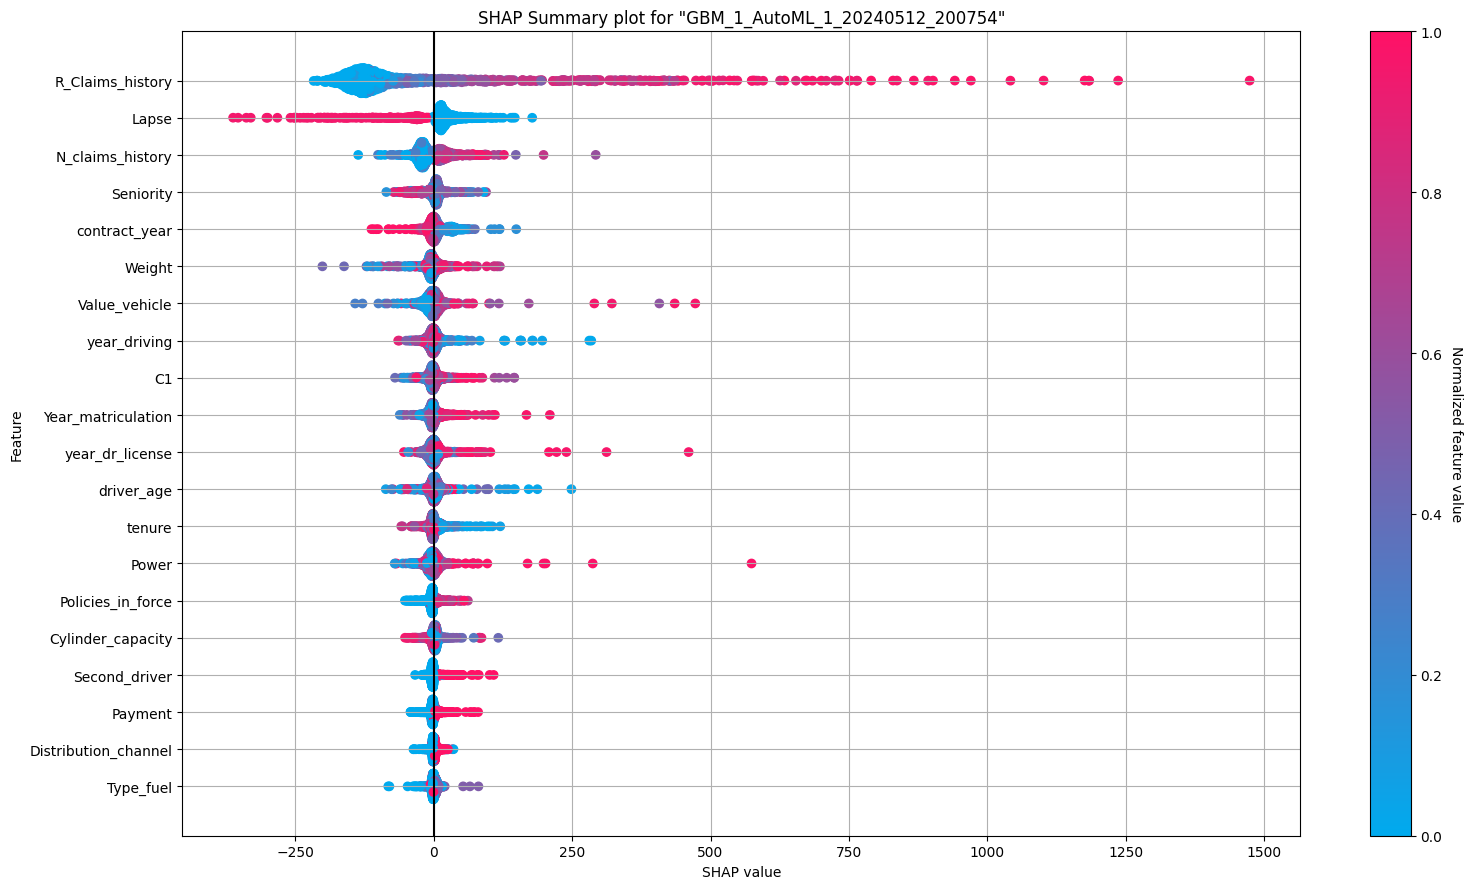
\includegraphics[scale=0.4]{shap_plot.png}
\caption{Shapley Plot}
\label{fig:univerise}
\end{figure}

Explain what is Shapeley value 

How to use Shapeley Plot?



\section{Potential Risks and How to Manage Them}

\begin{itemize}
    \item 
    \item Outlier detection
    \item 
    \item 
\end{itemize}


\section{Conclusion}



\bibliographystyle{plain}
\bibliography{references}
\end{document}
